\documentclass{config/apuntes}

\title{Procesado y Manejo de Datos Masivos}
\author{Sandra Mingo Ramírez}
\date{2024/25}
\acronym{PRMDM}

\usepackage[all]{nowidow}
\usepackage{listing}
\usepackage{color}
\usepackage{tabularx}
\usepackage{multirow}
\usepackage{makecell}
\usepackage{amsmath}
\usepackage{array}

\definecolor{dkgreen}{rgb}{0,0.6,0}
\definecolor{gray}{rgb}{0.5,0.5,0.5}
\definecolor{mauve}{rgb}{0.58,0,0.82}

\lstset{
  frame=tb,
  aboveskip=3mm,
  belowskip=3mm,
  showstringspaces=false,
  columns=flexible,
  basicstyle={\small\ttfamily},
  numbers=none,
  numberstyle=\tiny\color{gray},
  keywordstyle=\color{blue},
  commentstyle=\color{dkgreen},
  stringstyle=\color{mauve},
  breaklines=true,
  breakatwhitespace=true,
  tabsize=3
}

\begin{document}

\begin{abstract}
En esta asignatura se aprenderán técnicas para procesar y manipular grandes volúmenes de datos utilizando programación y línea de comandos. Se abordará el manejo y análisis de formatos de datos comunes en bioinformática, como FASTA, GFF y GenBank, utilizando patrones que optimizan el uso de memoria y tiempo de ejecución, así como técnicas de programación paralela. Además, se realizarán operaciones avanzadas en bases de datos relacionales y no relacionales, y se explorará el acceso programático a bases de datos biomédicas online a través de sus APIs.
\end{abstract}

\pagestyle{plain}

\maketitle

\tableofcontents

%Se han invertido los temas y su orden: primero daremos herramientas de programación, y luego ya Linux
%Se trabaja en Linux principalmente, incluido Python (aunque funciona igual en Windows)
%3 bloques:
%		Uso práctico de la línea de comandos para la extracción y correlación de información
% 	Estrategias programáticas de parseo y extracción de datos
%		Bases de datos
%08/10 - Gonzalo Martínez
\chapter{Estrategias de programación para el parseo y extracción de datos}
\section{Formatos de ficheros bioinformáticos}
Los formatos de fichero son en formato texto, y los principales son:
\begin{itemize}
\item \underline{FASTA}: guarda secuencia de nucleótidos o aminoácidos.
\item \underline{FASTQ}: conjunto de secuencias de nucleótidos leídas junto con sus puntuaciones de calidad
\item \underline{GFF/GTF}: formato de anotación de características del genoma
\item \underline{GenBank}: formato enriquecido para secuencias de nucleótidos o aminoácidos.
\end{itemize}

\subsection{FASTA}
Guarda una o varias secuencias de nucleótidos o aminoácidos. Se pronuncia como "fast A", que significa "fast all", siendo all cualquier alfabeto. Los archivos fasta pueden tener las siguientes extensiones:
\begin{itemize}
\item \textbf{.fasta, .fa}: extensión FASTA genérica
\item \textbf{.fna}: contiene secuencia de nucleótidos
\item \textbf{.faa}: contiene secuencia de aminoácidos
\item \textbf{.frn}: contiene secuencias de ARN no codificante
\end{itemize}

En la figura \ref{fig:fasta} se puede ver la estructura de un fichero FASTA. Cada secuencia consiste en una línea descriptiva seguida de las líneas que contienen la secuencia. La línea descriptiva cuenta con un símbolo > seguido del identificativo de la secuencia. Tras un espacio, se pone la descripción de la secuencia. En algunos casos, las secuencias se encuentran en mayúscula, en minúscula o en una mezcla de ambas. Por ello, se puede pasar toda la secuencia a mayúsculas o minúsculas con .upper() y .lower() respectivamente.

\begin{figure}[htbp]
\centering
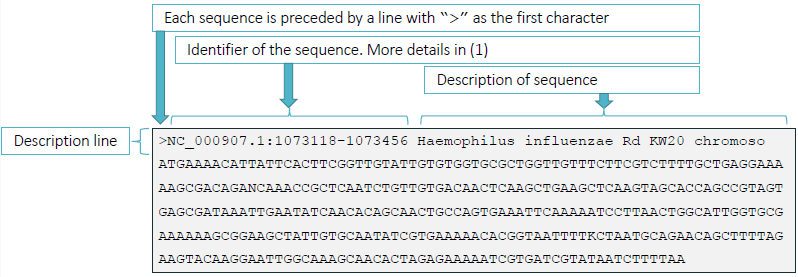
\includegraphics[width = \textwidth]{figs/fasta.png}
\caption{Anatomía de un fichero FASTA}
\label{fig:fasta}
\end{figure}

La secuencia se puede expandir por múltiples líneas, las cuales generalmente tienen unos 80 caracteres. No hay espacios en las líneas o líneas en blanco en una secuencia. Cada elemento de una secuencia se describe con un único carácter, y normalmente se escriben en mayúscula (aunque esto es una convención, no es estándar). No es recomendable utilizar guiones para representar gaps, ya que hay algunos programas que no los pueden manejar. Es mejor utilizar una N en el caso de secuencias de nucleótidos y X de aminoácidos (véase tabla \ref{tab:fasta-data}).

\begin{table}[htbp]
\centering
\begin{tabular}{l l l}
\multicolumn{3}{c}{\textbf{FASTA for genome data}}\\
A adenosine & C cytidine & G guanine \\
T thymidine & N A/G/C/T (any) & U uridine \\
K G/T (keto) & S G/C (strong) & Y T/C (pyrimidine) \\
M A/C (amino) & W A/T (weak) & R G/A (purine)\\
B G/T/C & D G/A/T & H A/C/T \\
V G/C/A & - gap & \\ \\ \hline \\
\multicolumn{3}{c}{\textbf{FASTA for protein data}}\\
A alanine & B aspartate/asparagine &  C cystidine\\
D aspartate & E glutamate & F phenylalanine\\
G glycine & H histidine & I isoleucine \\
K lysine & L leucine & M methionine \\
N asparagine & P proline & Q glutamine\\
R arginine & S serine & T threonine\\
U selenocysteine & V valine & W tryptophan\\
Y tyrosine & Z glutamate/glutamine & X any \\
* translation stop & - gap \\
\end{tabular}
\caption{Caracteres en los ficheros FASTA para datos genómicos y de proteínas.}
\label{tab:fasta-data}
\end{table}

\subsubsection{Parsear ficheros FASTA en Python}
En informática, parsear significa leer un fichero. Se pueden leer ficheros FASTA en Python de la siguiente forma:
\begin{lstlisting}[language=Python]
def readFasta(file):
    """ Reads all sequences of a FASTA file 
        returns a dictionary """  
    d = {}
    identifier = ''
    
    with open(file, 'r') as f:
        for linea in f:
            if linea[0] == ">": #alternativa: linea.startswith(">")
                if identifier != '':
                    d[identifier] = ''.join(d[identifier])
                descriptors = linea[1:].split()
                identifier = descriptors[0]
                #Alternativa: identifier = linea[1:linea.find(' ')]
                d[identifier] = []
                
            else:
                d[identifier].append(linea.strip('\n'))
        d[identifier] = ''.join(d[identifier])
    return d

readFasta("phix174/phix.fa")
\end{lstlisting}

\subsection{FASTQ}
Los ficheros FASTQ guardan secuencias de nucleótidos junto con las calidades.

Cada secuencia de un archivo FASTQ consta de 4 líneas. La primeras es la línea de descripción precedida de \@. Tiene un formato libre sin límite de longitud. A veces se coloca un identificador justo después de la \@. La segunda línea es la línea de secuencia, e incluye la secuencia propiamente dicha. Sigue normas y convenciones similares a las del fichero FASTA: normalmente en mayúsculas, sin espacios permitidos, etc. Esta línea podría estar envuelta en múltiples líneas como en un archivo FASTA. La siguiente es la línea que señala el final de la secuencia. Está marcada con el signo +. Puede ir seguida de la misma descripción dada en la primera línea. Sin embargo, es más sensato dejarla sólo con el '+' para reducir el tamaño de los ficheros. La última línea es la línea de puntuaciones de calidad: una secuencia codificada en caracteres con la calidad de las lecturas de la secuencia. Contiene un carácter por base. Los caracteres permitidos son como máximo ASCII 33-126 inclusive, que son todos imprimibles. Esta línea puede ser envuelta como en un archivo FASTA y su longitud total debe ser igual a la secuencia. Véase un ejemplo de un archivo FASTQ en la figura \ref{fig:fastq}.

\begin{figure}[htbp]
\centering
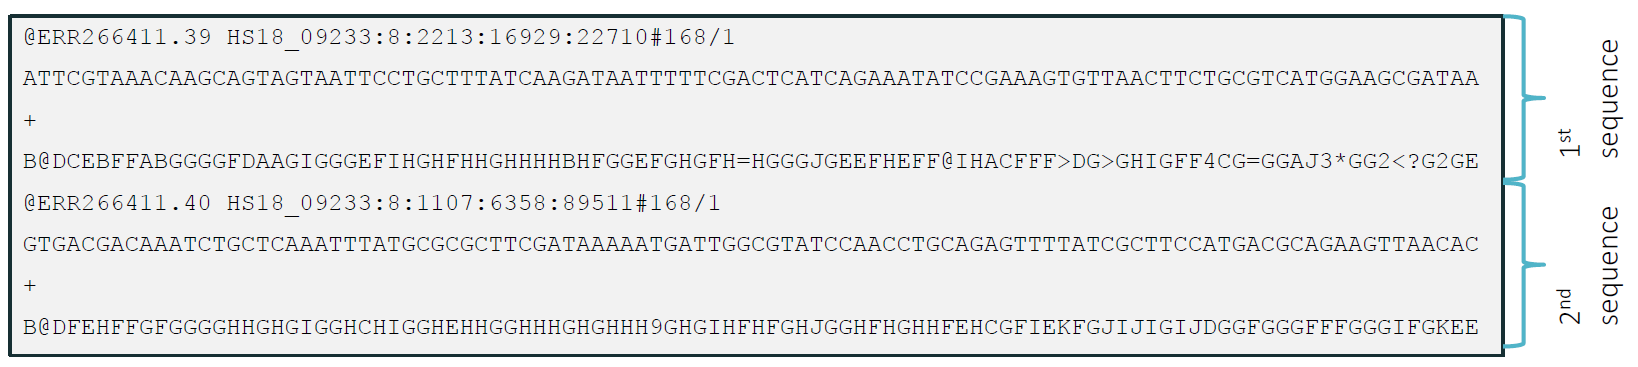
\includegraphics[width = \textwidth]{figs/fastq.png}
\caption{Anatomía de un fichero FASTQ}
\label{fig:fastq}
\end{figure}

Hay varias cuestiones que deben tenerse en cuenta al analizar un archivo FASTQ: Tanto el carácter \@ como + pueden aparecer en la línea con los índices de calidad. Pueden aparecer en la primera posición, por lo que hay que tener cuidado al utilizar grep o herramientas similares: por ejemplo \texttt{ \$> grep -v "[\@ +]" file.fastq} (Este comando para eliminar las líneas + y \@ no es una buena idea). En principio, tanto la secuencia como las puntuaciones de calidad pueden tener múltiples saltos de línea. El programa de análisis debería eliminar los saltos de línea. Para reducir los problemas de análisis sintáctico, la mayoría de las herramientas producen ahora archivos fastq en los que las secuencias y las puntuaciones de calidad se dan en una sola línea, posiblemente muy larga. Por lo tanto, cada secuencia tiene exactamente 4 líneas, lo cual es conveniente.

La codificación más utilizada para las puntuaciones de calidad es el formato Sanger o codificación Phred+33. Cada carácter codifica la calidad de la lectura, Q, que se define como:
$$Q = -10 \cdot log_{10} p$$
siendo p la probabilidad de error de la lectura. Esta puntuación de calidad se utiliza porque permite una interpretación fácil de la probabilidad (Q = 10, p = 1/10; Q = 20, p = 1/100; Q = 30, p = 1000) y porque permite una codificación en un único carácter ASCII. No obstante, no se puede guardar Q directamente como un carácter porque no todos son imprimibles. Por ello, se emplea la codificación Phred+33, que codifica el valor Q como:
$$Q = ord(chr) - 33$$
donde ord() convierte el carácter a su representación ASCII. Por ejemplo, el símbolo \@ tiene el código ASCII de 64, por lo que su Q sería de 31. Una p de 0 significa que es una lectura segura, mientras que una p de 1 indica que la lectura no es nada segura. Para calcular la p, se despeja la fórmula para que quede:
$$ p = 10^{-\frac{Q}{10}}$$

\textbf{Ejemplos:}
Para el carácter "~", el código ASCII es 126, por lo que su Q es $126-33 = 93$. En este caso, la p sería de $0,5 \cdot 10^{-10}$ .  Así, el carácter "!", cuyo ASCII es 33, tiene una Q de 0 y una p de 1. 

En este caso, como las letras en mayúscula y minúscula tienen un código ASCII diferente, no se puede pasar todo a mayúsculas o minúsculas como en FASTA.

\subsection{GFF: generic feature format}
Los ficheros GFF tienen un formato de texto sin formato para representar características genómicas. Cada característica está representada por nueve columnas separadas por tabuladores:
\begin{enumerate}
\item \underline{seqid}: id de la secuencia donde se localiza la característica. No se permiten espacios
\item \underline{source}: nombre del programa o algoritmo que ha generado esta característica.
\item \underline{type}: tipo de característica (region, gene, CDS, etc.)
\item \underline{start}: posición donde inicia la característica, su primera base
\item \underline{end}: posición donde finaliza la característica, su última base
\item \underline{score}: un valor flotante que indica la confianza en la característica. Si no se conoce, se pone un punto.
\item \underline{strand}: indica el sentido de la cadena, siendo + la cadena positiva y - la cadena negativa.
\item \underline{phase}: puede ser 0, 1 o 2 para CDS y un punto para todo lo demás. 
\item \underline{attributes}: Una lista de atributos de la característica en formato tag=value separados por punto y coma (;). Se permiten espacios en blanco en estas columnas, así como tabuladores y punto y coma si se escapan. Los atributos son:
\begin{itemize}
\item \textbf{ID}: El id de la característica. Debe ser único dentro del archivo gfffile. Tenga en cuenta que para las características no contiguas el id puede aparecer en varias líneas. Se considera una característica única
\item \textbf{Name}: Nombre de la característica. No es necesario que sea único.
\item \textbf{Parent}: Id del elemento padre. Indica la relación «parte de». Un elemento puede tener varios padres. En este caso, los identificadores se separan por comas.
\item \textbf{Note}: nota de texto libre
\item \ldots
\end{itemize}
\end{enumerate}

\begin{figure}[htbp]
\centering
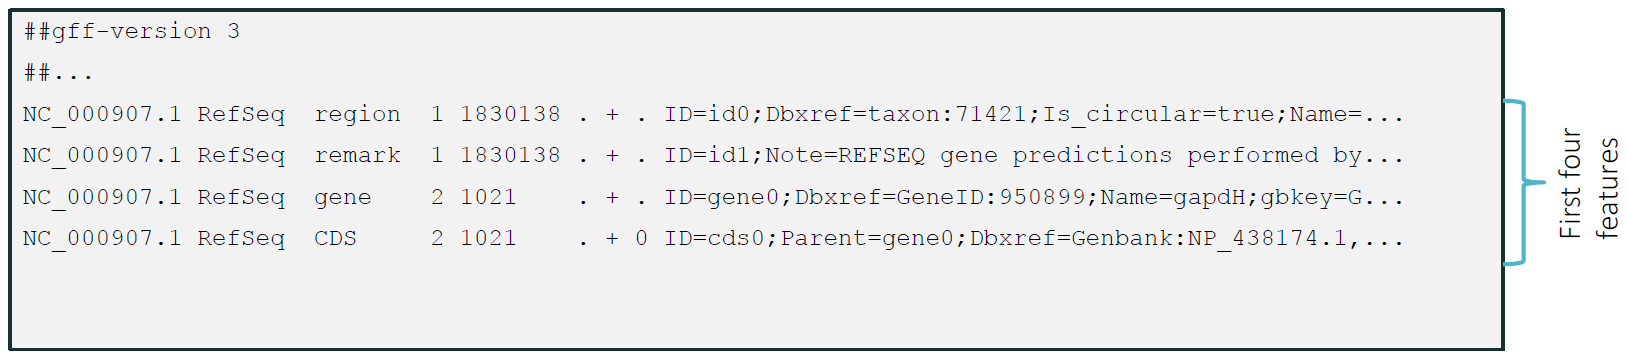
\includegraphics[width = \textwidth]{figs/gff.png}
\caption{Primeras columnas de un fichero GFF.}
\label{fig:gff}
\end{figure}

Hay varias cuestiones que deben tenerse en cuenta al analizar un archivo GFF: Las columnas sólo están separadas por tabuladores, pero se permiten espacios en blanco en algunos campos. Por tanto, hay que tener cuidado con grep y herramientas shell similares. Algunos caracteres se escapan en algunos campos, es decir, no queremos que los caracteres se interpreten como los caracteres que son. Esto ocurre con los puntos y coma y los espacios. Estos caracteres se escriben de otra forma; por ejemplo, un valor de a en punto y coma debe codificarse con \%3B. Para decodificar estos caracteres puede utilizar urllib. Además, una fila con triple almohadilla (\#\#\#) indica que se han resuelto todas las características multilínea hasta ese punto. Hay al menos una de estas líneas al final del fichero. Las líneas que empiezan por \# son comentarios. La región definida por los rasgos CDS incluye los codones de inicio y fin.

\begin{figure}[htbp]
\centering
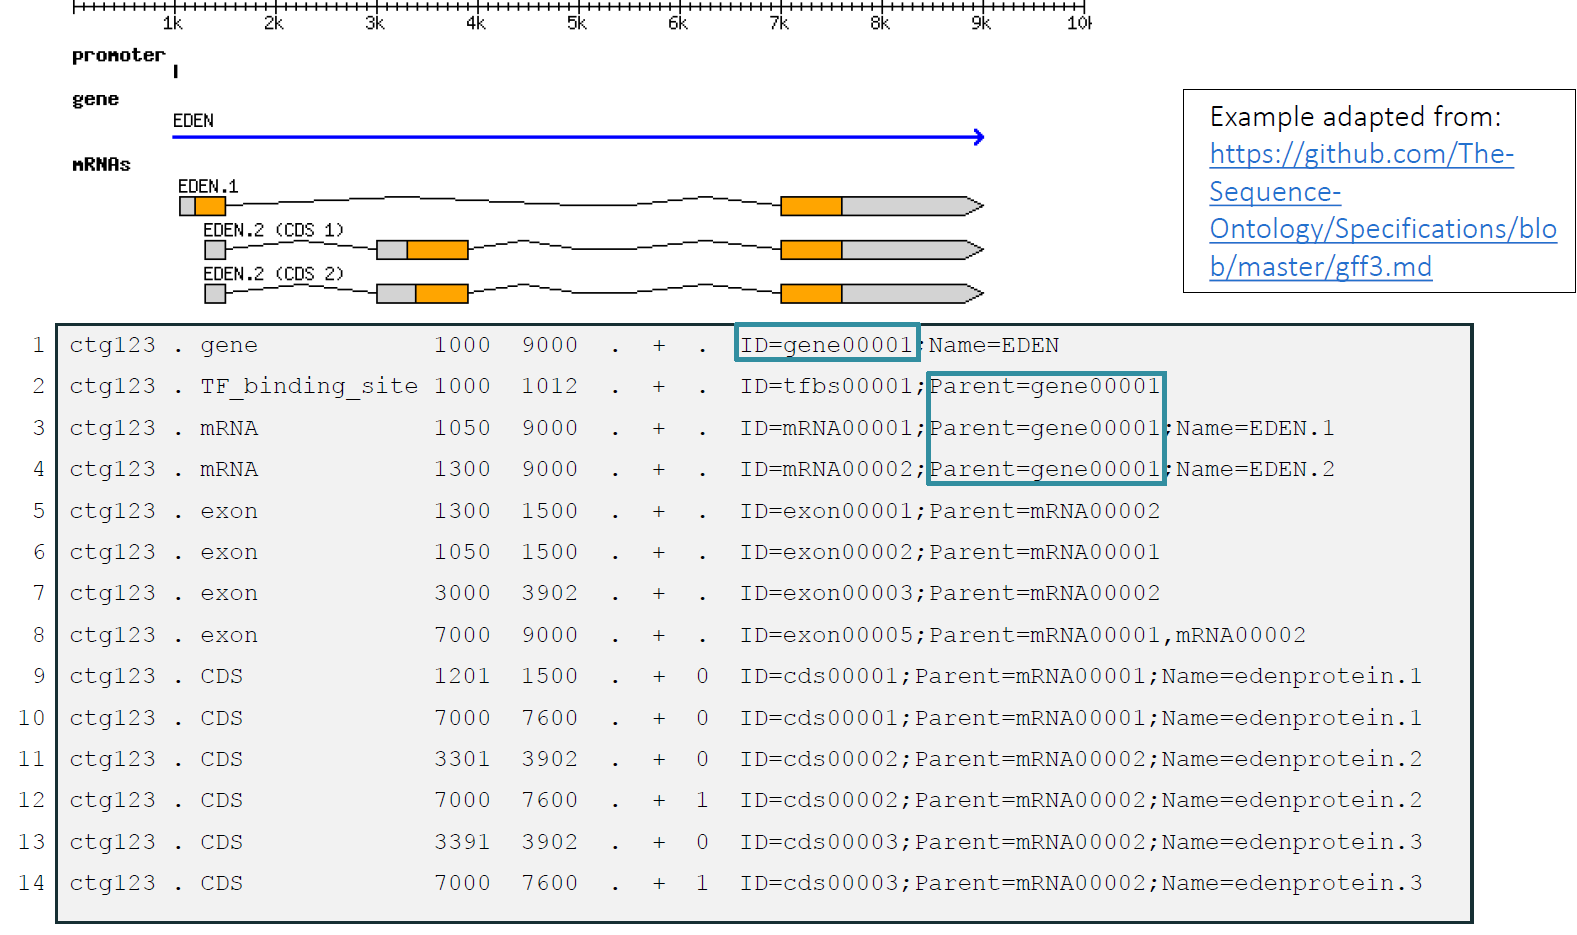
\includegraphics[width = \textwidth]{figs/gff-graph.png}
\caption{Ejemplo gráfico de una región genómica con el fichero GFF.}
\label{fig:gff-graph}
\end{figure}

Se puede trabajar con un fichero GFF desde la terminal de Linux. Por ejemplo, se pueden buscar todas las regiones (\texttt{grep region fichero.gff}) u obtener las terceras columnas (\texttt{cut -f3 fichero.gff}).

\begin{lstlisting}[language=Python]
def readGFF(file):
    """ Counts region types of a GFF file 
        returns a dictionary """  
    d = {}
    
    with open(file, 'r') as f:
        for linea in f:
            if linea[0] != "#": 
                campos = linea.split("\t")
                region_type = campos[2]
                if region_type not in d: #o d.keys()
                    d[region_type] = 1
                else:
                    d[region_type] += 1
    return d

readGFF('data/haemophilus_influenzae/GCF_000027305.1_ASM2730v1_genomic.gff')
\end{lstlisting}

\subsection{GenBank record}
GenBank es una base de datos de secuencias de libre acceso mantenida por el National Center for Biotechnology Information (NCBI). Esta base de datos tiene un formato de archivo plano para representar un registro en la base de datos. Este formato codifica la secuencia, las características y las referencias de proteínas y genes.

\begin{figure}[htbp]
\centering
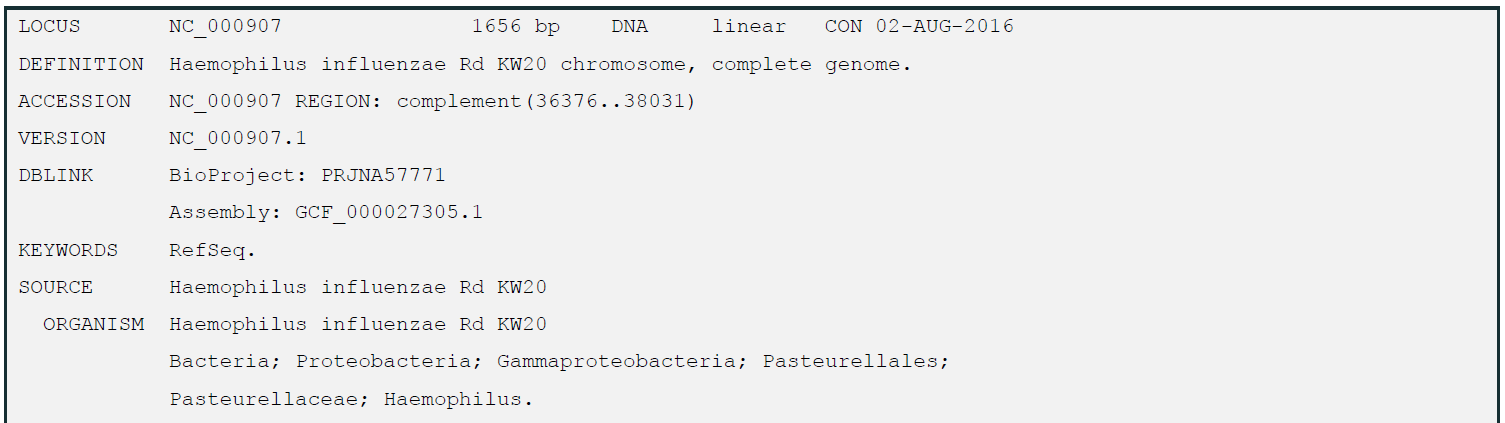
\includegraphics[width = \textwidth]{figs/genbank.png}
\caption{Principio de un documento GenBank.}
\label{fig:genbank}
\end{figure}

Las partes de un documento GenBank (figura \ref{fig:genbank}) son:
\begin{itemize}
\item LOCUS: Contiene un identificador (NC\_000907 en el ejemplo siguiente), la longitud de la secuencia (1656 pb), el tipo de molécula (ADN) y la fecha de la última modificación del registro.
\item DEFINITION: Breve descripción de la secuencia.
\item ORGANISM: Nombre científico del organismo .
\item REFERENCE: Publicación científica relacionada con la secuencia. La última suele referirse al autor que envió la secuencia (esta referencia se marca con «direct submission» en lugar del título del artículo).
\item FEATURES: Información sobre genes y productos génicos de la secuencia. Tiene varios subcampos:
\begin{itemize}
\item Source: Campo obligatorio que describe la longitud y el organismo de la secuencia.
\item gene: región de un gen
\item CDS: región codificante de una proteína. Incluye translation, tabla, protein\_id, producetname, notas, etc.
\end{itemize}
\end{itemize}

\section{Librerías de Python}
\subsection{NumPy}
NumPy (Numerical Python) es una librería de Python que permite realizar operaciones con arrays y matrices. También incluye herramientas de álgebra lineal, estadística o generación aleatoria de números. Se combina frecuentemente con otras librerías como SciPy para computaciones numéricas y pandas para análisis de datos.

\subsubsection{Clase ndarray}
\paragraph{Creación de arrays}
El elemento principal de NumPy es el objeto \textbf{ndarray} que representa arrays multidimensionales. Es capaz de realizar operaciones vectoriales eficientes (en velocidad y memoria). Al contrario que las listas de Python, todos los elementos de un ndarray son del mismo tipo. Los tipos posibles son int, float, boolean, string, etc. El atributo shape te da el tamaño del array y dtypet el tipo de los elementos.
\begin{lstlisting}[language=Python]
import numpy as np

data = np.array([[1, 2, 3], [4, 5, 6], [7, 8, 9]])
data.shape 
#Output: (3, 3)
data.dtype
#Output: dtype('int64')
\end{lstlisting}

Se puede crear un array a partir de cualquier otra secuencia (listas u otros ndarrays), utilizando la función numpy.array. Es posible especificar en la construcción el tipo del array (dtype) y la dimensión. Las dimensiones son importantes para cuando haya que fusionar arrays, ya que deberán coincidir. Además, la dimensión debe coincidir en todo el array, es decir, debe ser homogéneo.
\begin{lstlisting}[language=Python]
x = np.array([1, 2, 3], ndmin = 2)
# array([[1, 2, 3]])
y = np.array([1, 2], dtype = 'int32')

error = np.array([1, 2, 3], [4, 5])
\end{lstlisting}

Otras funciones para crear e inicializar arrays/matrices son:
\begin{itemize}
\item Matrices de ceros: numpy.zeros y numpy.zeros\_like (el primero crea un array de las dimensiones dadas, el segundo crea un array como el que se le pasa, es decir, con sus dimensiones y el tipo).
\item Matrices de unos: numpy.ones y numpy.ones\_like
\item Matriz identidad: numpy.eye y numpy.identity
\item La función numpy.arange se comporta de forma similar a la función estándar de python range, pero devuelve un ndarray.
\item La función numpy.linspace devuelve números espaciados uniformemente en un intervalo especificado. Se proporciona el primer y último valor y el número total de valores. La función numpy.logspace hace algo similar pero de forma logarítmica.
\end{itemize}

\begin{lstlisting}[language=Python]
np.zeros((3,2))
#array([[0., 0.], [0., 0.], [0., 0.]])

x = np.array([1, 2, 3])
np.ones_like(x)
#array([1, 1, 1])

y = np.arange(10)
#[0 1 2 3 4 5 6 7 8 9]

np.linspace(-np.pi,np.pi,10)
#array([-3.14159265, -2.44346095, -1.74532925, -1.04719755, -0.34906585, 0.34906585,  1.04719755,  1.74532925,  2.44346095,  3.14159265])
\end{lstlisting}

\paragraph{Operaciones básicas con arrays}
Las operaciones aritméticas pueden realizarse con ndarrays utilizando la misma sintaxis que la empleada para los escalares y evitando el uso de bucles explícitos. 
\begin{lstlisting}[language=Python]
data = np.array([[1, 2, 3], [4, 5, 6]])
data + 1
#array([[2, 3, 4], [5, 6, 7]])
data * 10
array([[10, 20, 30], [40, 50, 60]])
\end{lstlisting}

Arrays del mismo tamaño se pueden sumar y multiplicar celda a celda (si son de distinto tamaño no funciona):
\begin{lstlisting}[language=Python]
data + data
#array([[ 2,  4,  6], [ 8, 10, 12]])
data * data
#array([[ 1,  4,  9], [16, 25, 36]])
\end{lstlisting}

Todas las operaciones booleanas (>, <, ==, etc) se aplican elemento a elemento y se devuelve un array de booleanos:
\begin{lstlisting}[language=Python]
data = np.array([[1, 2, 3], [4, 5, 6], [4, 5, 6]])
#array[[1 2 3], [4 5 6], [4 5 6]]
data > 4
#array([[False, False, False], [False,  True,  True], [False,  True,  True]])
\end{lstlisting}

\paragraph{Ejercicios}
Construye una matriz de 5x5 elementos en la que los elementos de la diagonal sean 10  y los elementos fuera de la diagonal sean 5.
\begin{lstlisting}[language=Python]
np.identity(5)*5+5
(np.identity(5)+1)*5

def diag2(n, f):
	''' f: factor, n: dimensiones del array'''
	return (np.identity(n) + 1) * f
diag2(5,5)
\end{lstlisting}

Crea un array que contenga los días de la semana. ¿Cuál es su dtype?
\begin{lstlisting}[language=Python]
weekdays_matrix = np.array(['Monday', 'Tuesday', 'Wednesday', 'Thursday', 'Friday', 'Saturday', 'Sunday'])
print(weekdays_matrix.dtype)
#<U9
#El 9 es la longitud de palabra más grande del array
\end{lstlisting}

\subsubsection{Indexación y slicing}
Para arrays unidimensionales, el funcionamiento es como en el caso de las listas:
\begin{lstlisting}[language=Python]
x = np.arange(10)
#array([0, 1, 2, 3, 4, 5, 6, 7, 8, 9])
x[4] 
#4
x[2:7]
#array([2, 3, 4, 5, 6])
x[-3:]
#array([7, 8, 9])
\end{lstlisting}

Si se asigna un valor a un slice, el valor se asigna a todas las posiciones en el slice.
\begin{lstlisting}[language=Python]
x[4:7] = -1
#array([ 0,  1,  2,  3, -1, -1, -1,  7,  8,  9])
x = np.arange(10)
#array([0, 1, 2, 3, 4, 5, 6, 7, 8, 9])
x[0::2] = [19,17,15,13,11]
#array([19,  1, 17,  3, 15,  5, 13,  7, 11,  9])
\end{lstlisting}

Ten en cuenta que si obtienes una referencia a un slice, los elementos no se copian y sólo se mantiene la referencia a los elementos del slice. Esto significa que si después utilizas el slice para modificar sus valores, éstos se modifican en el array original. Si queremos una copia del slice y no una referencia a los valores en los arrays originales, se puede utilizar el método copy().
\begin{lstlisting}[language=Python]
x = np.ones((5,3), dtype=int)
#array([[1, 1, 1], [1, 1, 1], [1, 1, 1], [1, 1, 1], [1, 1, 1]])
y = x[:5:2,1:] #aquí se seleccionan primero filas y luego columnas
#array([[1, 1], [1, 1], [1, 1]])
y[:] = 25
print(x)
#array([[ 1, 25, 25], [ 1,  1,  1], [ 1, 25, 25], [ 1,  1,  1], [ 1, 25, 25]])

x = np.ones((5,3), dtype=int)
z = x[:3].copy()
#array([0, 1, 2])
y[2] = 25
print(x)
#[0 1 2 3 4 5 6 7 8 9]
print(y)
#[ 0  1 25]
\end{lstlisting}

En arrays multidimensionales, se utilizan comas para separar los slices para cada dimensión.
\begin{lstlisting}[language=Python]
data = np.array([[1, 2, 3, 4], [5, 6, 7, 8], [9, 10, 11, 12], [13, 14, 15, 16]])
#array([[ 1,  2,  3,  4], 
# [ 5,  6,  7,  8], 
#[ 9, 10, 11, 12], 
#[13, 14, 15, 16]])
data[1,1:3]
#array([6, 7])
data[1:3]
#array([[ 5,  6,  7,  8], 
# [ 9, 10, 11, 12]])
data[:, 1:3]
#array([[ 2,  3],
# [ 6,  7],
# [10, 11],
# [14, 15]])
data[1:4:2, 1:4:2]
#array([[ 6,  8],
# [14, 16]])
\end{lstlisting}

\paragraph{Indexación booleana}
Es posible utilizar un array de valores booleanos (Verdadero/Falso) para seleccionar elementos del ndarray.
\begin{lstlisting}[language=Python]
data = np.random.randn(10, 3) #generación de matriz 10x3 con números de distribución normal
data[data>0] #números positivos
ix = data[:,0] > 0 #índices booleanos para las filas en las que el primer elemento es positivo
#array([ True,  True, False, False,  True, False, False, False, False, True])
selected = data[ix, :] #seleccionar las filas que empiezan por un número positivo
\end{lstlisting}

La indexación booleana siempre crea una copia, a diferencia del slicing. Es posible combinar varias operaciones booleanas utilizando \& (and), | (or) y $\sim$ (negación). Además, se puede utilizar para asignar valores a los elementos de un array que cumplan con una condición.
\begin{lstlisting}[language=Python]
data[(data[:, 0] > 0) & (data[:, 2] < 0), :] #selecciona las filas en las que el primer elemento es positivo y el último negativo
data[data < 0] = 0 #asigna el valor de 0 a todos los elementos negativos
\end{lstlisting}

\paragraph{Indexación fancy}
También es posible indexar utilizando matrices de enteros de forma similar al slicing. Estos enteros indican los índices de columna o fila a seleccionar. Este tipo de indexación es útil, por ejemplo, para seleccionar filas y columnas en un orden distinto al original.
\begin{lstlisting}[language=Python]
nrows = 5
ncols = 3
p = 1
data = np.zeros((nrows, ncols))
for i in range(ncols):
    data[:, i] = np.arange(nrows)*p
    p*=10
#array([[  0.,   0.,   0.],
#       [  1.,  10., 100.],
#       [  2.,  20., 200.],
#       [  3.,  30., 300.],
#       [  4.,  40., 400.]])
data[[3, 1]] #selección de las filas 3 y 1 en ese orden
#array([[  3.,  30., 300.],
#       [  1.,  10., 100.]])
data[:, [2, 0]]
#array([[  0.,   0.],
#       [100.,   1.],
#       [200.,   2.],
#       [300.,   3.],
#       [400.,   4.]])
\end{lstlisting}

\paragraph{Ejercicios} 
En el siguiente código, ¿qué diferencia supondría \texttt{y = 100 * y} con \texttt{y[:] = 100*y}?
\begin{lstlisting}[language=Python]
x = np.array([1, 2, 3, 4, 5])
y = x[:3]
y = 100*y
print(y) # [100 200 300]
print(x) # [1 2 3 4 5]
y = x[:3]
y[:] = 100*y
print(y) # [100 200 300]
print(x) # [100 200 300   4   5]
\end{lstlisting}
De ambas formas, el resultado para y es igual; la diferencia se encuentra en el array original x. En la primera variante, x no se ve modificado, mientras que en la segunda variante, los valores de x sí se han visto modificados.

%15/10 - Gonzalo Martínez
El siguiente array contiene una lista de 100 notas aleatorias de 0 a 10. Crea un array que tenga una nota cualitativa para cada nota numérica:
\begin{lstlisting}[language=Python]
n = 100
np.random.seed(13)
notas = np.random.rand(n)*10

notas_cual = np.array(notas, dtype=str)
notas_cual[notas < 5] = "SUSPENSO"
notas_cual[(notas >= 5) & (notas < 7) ] = "APROBADO"
notas_cual[(notas >= 7) & (notas < 9) ] = "NOTABLE"
notas_cual[notas >= 9] = "SOBRESALIENTE"
\end{lstlisting}

Ahora cuenta el número de suspensos, aprobados, notables y sobresalientes.
\begin{lstlisting}[language=Python]
np.sum(notas_cual == "SUSPENSO")
np.sum(notas_cual == "APROBADO")
np.sum(notas_cual == "NOTABLE")
np.sum(notas_cual == "SOBRESALIENTE")
\end{lstlisting}

Hay más funciones de Numpy que no hemos visto. Por ejemplo, \texttt{np.unique} proporciona todos los valores únicos. Así, el ejercicio anterior se podría resolver de la siguiente forma:
\begin{lstlisting}[language=Python]
for value in np.unique(notas_cual):
    print("# de ", value, ":", np.sum(notas_cual == value))
\end{lstlisting}
\subsubsection{Operaciones con arrays}
\paragraph{Transponer}
La función \texttt{transpose} o \texttt{T} permite intercambiar las filas por columnas de un array. 
\begin{lstlisting}[language=Python]
data = np.array([[1, 2, 3, 4], [5, 6, 7, 8], [9, 10, 11, 12], [13, 14, 15, 16]])
data.T # o data.transpose()
\end{lstlisting}

También es posible transponer arrays multidimensionales especificando los índices de los ejes que se quieren intercambiar. 

\paragraph{Cambiar la forma de un array (reshape y ravel)}
El método \texttt{ndarray.reshape()} cambia la forma de un array sin cambiar su contenido, solo lo reajusta. El número de celdas totales en ambos arrays debería ser igual. El método \texttt{ndarray.ravel()} comprime un array en uno de una sola dimensión. Además, el método \texttt{np.concatenate} concatena dos arrays a lo largo de un eje, dado que el tamaño de la otra dimensión sea igual. Algunos ejemplos son:
\begin{lstlisting}[language=Python]
x = np.arange(1, 13) 
print(x)
y = x.reshape(3, 4) #cambia a dimensiones 3x4
print(y)
z = y.ravel() #vuelve a 1 dimensión
print(z)

x = np.zeros((3, 4))
print(x)
y = np.ones((3, 2))
print(y)
np.concatenate((x, y), axis = 1) #el eje 1 son las columnas
np.concatenate((x[:, :2], y), axis = 0) #eje 0 son las filas, y sólo se obtienen las primeras dos columnas de x
\end{lstlisting}

\subsection{Matplotlib}
Matplotlib es una librería de gráficos. Se suele importar como \texttt{import matplotlib.pyplot as plt}. La función más sencilla es \texttt{plot}.
\begin{lstlisting}[language=Python]
x = np.linspace(0.1, 4, 40) #[0.1, 0.2, 0.3, 0.4, 0.5, ...]
y = 1/x #[10., 5., 3.3333, 2.5, 2., ...]
plt.plot(x, y)
\end{lstlisting}

También se pueden imprimir varias líneas a la vez:
\begin{lstlisting}[language=Python]
x = np.linspace(-np.pi, np.pi, 40) 
y1 = np.sin(x)
y2 = np.cos(x)
# Use dummy variable _ to get the return value of plot to avoid printing its reference
_ = plt.plot(x, y1, x, y2)
\end{lstlisting}

\paragraph{Opciones de trazado}
Se puede especificar la forma de trazado al proporcionar una cadena que incluya un identificador. 
\begin{lstlisting}[language=Python]
x = np.arange(0.1,4,0.1)
y = 1/x
plt.plot(x, y, 'm*')
\end{lstlisting}
En el caso anterior, m representa el color magenta y el asterisco la forma de cada punto en el gráfico. Así, las líneas discontinuas se muestran como dos guiones, guion punto alterna ambos símbolos, la k representa el color negro, etc. Todas las opciones se pueden encontrar en \href{https://matplotlib.org/stable/api/_as_gen/matplotlib.axes.Axes.plot.html#matplotlib.axes.Axes.plot}{la guía}.

También se pueden retocar otras propiedades:
\begin{itemize}
\item linewidth: el ancho de la línea en píxeles
\item markeredgecolor: el color del borde del marcador
\item markerfacecolor: el color interno del marcador
\item markerzie: el tamaño del marcador
\end{itemize}
En general, estos parámetros aplican a todo el gráfico. Sin embargo, se puede establecer anchos y colores distintos para cada una de las líneas llamando al plot varias veces:
\begin{lstlisting}[language=Python]
x  = np.arange(0.1,20,0.5)
y  = np.exp(0.1*x)
y1 = y * np.sin(x)
y2 = y * np.cos(x)

_ = plt.plot (x, y1, ':ms', linewidth=2, markeredgecolor='k', markerfacecolor='r', markersize=5)
_ = plt.plot (x, y2, '-co', linewidth=11, markeredgecolor='b', markerfacecolor='c', markersize=11)
\end{lstlisting}

\paragraph{Tipos de gráficos}
Se pueden crear distintos tipos de gráficos:
\begin{itemize}
\item Gráfico de tarta (pie plot): mediante \texttt{plt.pie(x, Explode)}, siendo Explode la distancia a la que se debe separar la fracción.
\item Histograma: \texttt{hist(x, nbins)}. Por defecto, se crean 10 cajas o bins equidistantes. Si x es una matriz, entonces se crea un histograma por columna.
\item Diagrama de barras (bar plot): la función \texttt{bar(x, y, width, bottom, style...} crea un gráfico de barras verticales u horizontales (\texttt{barh}). El parámetro width indica la separación entre las barras, y bottom permite poner barras apiladas.
\item Contour: Esta función \texttt{contour(Z, n)} traza isolíneas desde la matriz Z, donde Z se interpreta como alturas con respecto al plano xy. Z debe ser al menos una matriz de 2x2. El número de niveles puede especificarse utilizando el parámetro «n»; de lo contrario, se calculan automáticamente a partir de las alturas máxima y mínima de Z.
\item Pcolor: La función \texttt{pcolor(c)} dibuja una matriz coloreada con colores dados por C. El gráfico muestra una columna y una fila menos que las columnas y filas de la matriz. Esta función (si no se dan otros parámetros) obtiene el color para la celda (i, j) del elemento (i, j) de la matriz C usando el mapa de colores actual.
\item Diagrama de dispersión (scatter plot): La función \texttt{scatter(x, y, s = 20, c=u'b', ...} crea un diagrama de dispersión con coordenadas x e y. Los vectores x e y deben tener el mismo tamaño. El tamaño de los puntos puede especificarse con s y su color con c. Tanto el tamaño como el color pueden darse para todos los puntos juntos utilizando un único valor o para cada punto individual utilizando un vector. Para la primera configuración, basta con dar un único escalar para el tamaño y una cadena para el color. Para la segunda, se debe dar un vector del mismo tamaño de x e y para los tamaños. Para los colores, se puede especificar un vector que contenga indixes f el mapa de colores, o un array de tamaño len(x) x 3 con colores en RGB.
\end{itemize}

\paragraph{Opciones globales para gráficos}
Todos los gráficos admiten una serie de funciones que permiten crear un gráfico "decente":
\begin{itemize}
\item figure: crea una figura del tamaño especificado. En esta opción también se puede especificar el color de fondo.
\item subplot(nrows, ncols): crea una matriz de gráficos de filas nrows y columnas ncols. El último parámetro indica sobre qué gráfico vamos a trabajar. También hay más parámetros como sharex o sharey que permite crear ejes compartidos entre todos los subgráficos. También se debe indicar mediante índice el subgráfico que se quiere modificar a continuación.
\item xlabel ylabel: permite indicar el nombre de los ejes x e y.
\item title: permite especificar el título del gráfico.
\item legend: añade la leyenda al gráfico. Se debe llamar esta opción una vez se haya ejecutado la función de creación del gráfico.
\item colorbar: incluye una barra de colores de referencia.
\item xlim ylim: modifica los límites de los ejes que se muestren en las gráficas.
\item xticks yticks: modifica las marcas de los ejes.
\end{itemize}
Un ejemplo de como aplicar todo esto sería el siguiente (el resultado se ve en la figura \ref{fig:plt1}):
\begin{lstlisting}[language=Python]
plt.figure(num=None, figsize=(12, 4), facecolor='c')

# Data
x = np.linspace(-np.pi,np.pi,20)
Y1 = np.sin(x)
Y2 = np.cos(x)

# Graph using legend and labels in the axis
plt.subplot(1,2,1) # Create a graph with two subplots. We start working on the first
plt.xlabel('x')
plt.ylabel('y')
plt.plot(x, Y1, label='sen')
plt.plot(x, Y2, label='cos')
plt.legend(loc=2) # Called after finishing the plot

# Graph with x label, title, with the limits of the axis modified
# and also the labels for the x axis
plt.subplot(1,2,2) # Now we use the second subplot
plt.xlabel('x')
plt.title('Seno y coseno')
plt.xlim([-3,3])
plt.xticks(range(-3,4), ['a','b','c','d','e','f','g'])
plt.plot(x, Y1, label='sen')
_ = plt.plot(x, Y2, label='cos')
\end{lstlisting}

\begin{figure}[htbp]
\centering
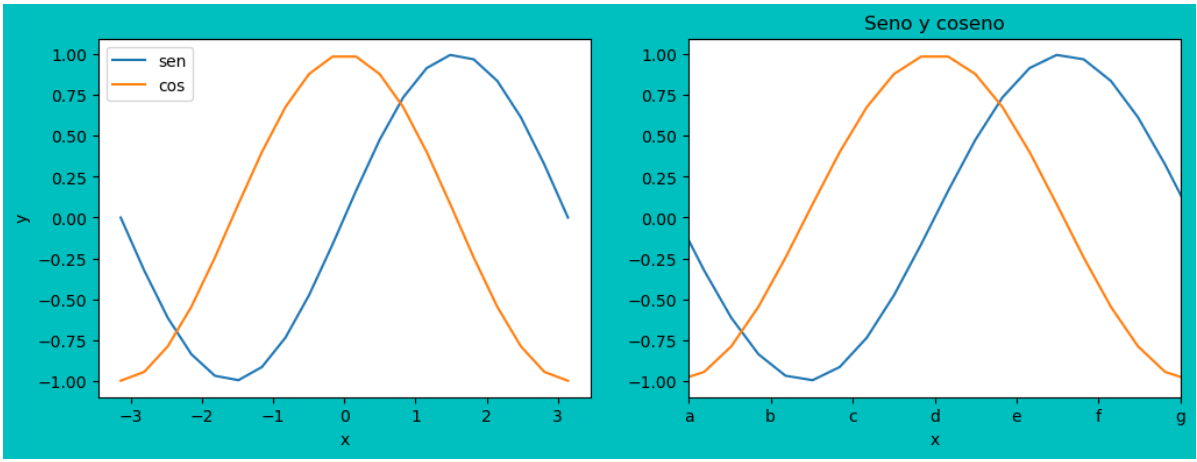
\includegraphics[width = \textwidth]{figs/plt1.png}
\caption{Gráfico de ejemplo}
\label{fig:plt1}
\end{figure}

Otro ejemplo sería:
\begin{lstlisting}[language=Python]
def sigmoid(V, V0, W=12):
    """ Sigmoidal function
    
    Parameters
    ----------
    V: float or array of floats
        Membrane potential
    V0: float
        Position of the sigmoid function
    W: float
        Width of the transition region
        
    Returns
    -------
    y: float or array of floats
        Sigmoidal function    
    """
    return 1/(1+np.exp(-(V-V0)/W))

V = np.arange(-100, 100, 1) #if we use linspace, instead of the steps we put how many values we want
y = sigmoid(V, -40, 12)

fig, axs = plt.subplots(1, 2)
#varying V0
ax = axs[0]
for V0 in [-40, 0, 40]:
    y = sigmoid(V, V0, 12)
    ax.plot(V, y, label = f'{V0:.0f}mV')
ax.set_xlabel('V [mV]')
ax.legend(title = '$V_0$')

#Varying W 
ax = axs[1]
for w in [1, 10, 20]:
    y = sigmoid(V, 0, w)
    ax.plot(V, y, label = f'{w:.0f}mV')
ax.set_xlabel('V [mV]')
ax.legend(title = '$w$')
plt.show()
\end{lstlisting}

\begin{figure}[htbp]
\centering
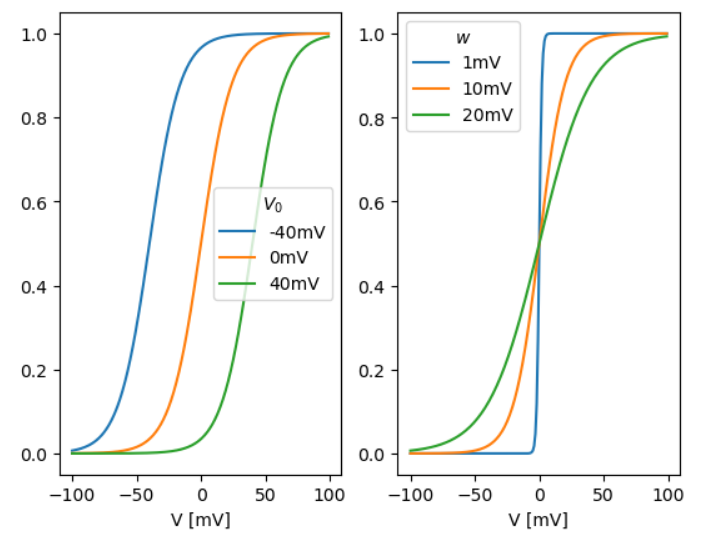
\includegraphics[width = 0.5\textwidth]{figs/plt2.png}
\caption{Otro ejemplo}
\label{fig:plt2}
\end{figure}

\section{Biopython}
Biopython es una librería Python con herramientas para computación biológica. Se trata de un proyecto de código abierto miembro de la Open Bioinformatics (OBF). Una fundación que promueve el código abierto en la investigación biológica.
El objetivo de esta librería es facilitar al máximo el uso de python en bioinformática para el análisis sintáctico de archivos, funciones para trabajar con secuencias y características, trabajar con sitios bioinformáticos online como NCBI o ExPASy, alineamientos, etc.

\subsection{Seq}
La clase Seq es la clase básica para representar secuencias en Biopython. Se representan las secuencias biológicas como cadenas. Así, se puede iterar sobre las bases, realizar slicing, concatenar secuencias y utilizar otros métodos de cadenas. Todas estas operaciones devuelven nuevos objetos de tipo Seq, que son inmutables, como los strings.

Esta clase tiene métodos especiales de ADN como \texttt{complement} o \texttt{reverse\_complement}. 
\begin{lstlisting}[language=Python]
dna = Seq('GATTACA')
print(dna.complement()) #CTAATGT
print(dna.reverse_complement()) #TGTAATC
\end{lstlisting}

También permite la transcripción mediante \texttt{transcribe} y \texttt{back\_transcribe} para obtener el ARN y la traducción para obtener la secuencia de aminoácidos (\texttt{translate}). Se puede especificar la tabla de traducción y si se desea parar justo antes del primer codón de stop.
\begin{lstlisting}[language=Python]
cds = Seq('GTGTTTTTGGTGTGGTGA')
mRNA = cds.transcribe()
print(mRNA) #GUGUUUUUGGUGUGGUGA
print(mRNA.back_transcribe()) #GTGTTTTTGGTGTGGTGA

mRNA = Seq('UUGUUUUUGGUGUGGUGA')

print("Translate using standard table: ", mRNA.translate()) #Translate using standard table:  LFLVW*
print("Translate until stop codon    : ", mRNA.translate(to_stop=True)) #Translate until stop codon    :  LFLVW
print("Using a different table       : ", mRNA.translate(table=2)) #Using a different table       :  LFLVWW
print("by name                       : ", mRNA.translate(table="Vertebrate Mitochondrial")) #by name                       :  LFLVWW
# This next line raises an error because the sequence is not a CDS for table=2
#print("CDS-like RNA                  : ", mRNA.translate(table=2, cds=True)) #CDS-like RNA                  :  MFLVW
# But it is a CDS-like sequence for table=11 (Bacterial)
print("CDS-like RNA                  : ", mRNA.translate(table=11, cds=True)) #CDS-like RNA                  :  MFLVW

cds = Seq('GTGTTTTTGGTGTGGTGA')
prot = cds.translate(table=11, cds=True)
prot = cds.translate()
prot #Seq('VFLVW*')
\end{lstlisting}

Si la secuencia es un CDS, debe tener un codón de inicio y final; si no, se produce un error. No es necesario seguir el flujo natural: se pueden obtener los aminoácidos directamente desde el ADN sin tener que pasar previamente por el ARN.

\subsubsection{Tablas de traducción}
Se pueden obtener las tablas de traducción:
\begin{lstlisting}[language=Python]
from Bio.Data import CodonTable

bacterial_table = CodonTable.unambiguous_dna_by_name['Bacterial']
print(bacterial_table)
\end{lstlisting}

\subsection{SeqRecord}
SeqRecord consta de una secuencia (objeto Seq) junto con id, descripción, anotaciones, características, etc. Se puede crear un SeqRecord a partir de un objeto Seq, de un archivo fasta, genbank, etc.
\begin{lstlisting}[language=Python]
from Bio.SeqRecord import SeqRecord

sr = SeqRecord(Seq('AAA'), id='1', description='Simple seq', annotations={"molecule_type": "DNA"})
print(sr)
\end{lstlisting}

\subsection{SeqIO}
IO viene de Input Output. 
Bio.SeqIO proporciona acceso a la mayoría de los formatos de archivos bioinformáticos.
La función \texttt{read()} carga un único archivo de secuencia. Obtiene como parámetros el nombre y formato del archivo.
Si hay más de un registro esta función genera un error. Esta función devuelve un SeqRecord.
\begin{lstlisting}[language=Python]
from Bio import SeqIO

record = SeqIO.read("phix174/phix.fa", "fasta")
print(record)
\end{lstlisting}

La función \texttt{parse} recupera varias secuencias de un archivo. Los parámetros son los mismos que read(): Nombre y formato del fichero. Esta función devuelve un iterador que permite recorrer todas las secuencias y puede iterar con un bucle
\begin{lstlisting}[language=Python]
for record in SeqIO.parse("other/ls_orchid.fasta", "fasta"):
    print(record)
    print()
\end{lstlisting}

Otra función es \texttt{to\_dict}, la cual crea un diccionario del iterador con todas las secuencias del fichero. El problema es que se guarda en la memoria, por lo que puede ralentizar el ordenador en caso de ficheros grandes.
\begin{lstlisting}[language=Python]
iterator = SeqIO.parse("other/ls_orchid.gbk", "genbank")
records_dict = SeqIO.to_dict(iterator)
print(records_dict['Z78533.1'])
\end{lstlisting}

La función \texttt{index()} crea un pseudo diccionario a partir de un fichero. Admite como parámetros el nombre y el formato del archivo. Esta función no almacena todo en memoria, sino que obtiene la información del disco cuando es necesario. Almacena la posición de cada secuencia en el fichero para un acceso rápido. Desde el punto de vista del usuario es como un diccionario de secuencias. Es importante cerrar el fichero cuando ya no se utilice.
\begin{lstlisting}[language=Python]
records_dict = SeqIO.index("other/ls_orchid.gbk", "genbank")
print(records_dict['Z78533.1'])
records_dict.close()
\end{lstlisting}

También se puede trabajar con ficheros comprimidos para ahorrar espacio en el disco:
\begin{lstlisting}[language=Python]
import gzip

with gzip.open("arabidopsis_thaliana/GCF_000001735.3_TAIR10_rna.fna.gz", "rt") as f:
    total_len = 0
    for sr in SeqIO.parse(f, "fasta"):
        total_len += len(sr.seq)
    print(total_len)
\end{lstlisting}

Trabajar con índices y archivos comprimidos es más complicado, ya que la posición de cada secuencia no es fácil de obtener. El formato Blocked GNU Zip Format ofrece una buena solución. Comprime los datos por bloques para permitir la indexación. La función Index() puede trabajar con el formato de archivo BGZF.

\subsection{Atributos de SeqRecord}
Los atributos más importantes de SeqRecord son:
\begin{itemize}
\item id y nombre: identificador y nombre de la secuencia
\item seq: objeto Seq que contiene la secuencia actual
\item annotations: diccionario de Python con toda la información de la secuencia. Se pueden encontrar tipos de moléculas, topología, fecha, accessiones, versión de secuencia, gi, palabras clave, fuente, organismo, taxonomía, referencias, etc.
\item features: lista de un objeto SeqFeature que contiene la información sobre las distintas características encontrada en una secuencia.
\end{itemize}
\begin{lstlisting}[language=Python]
records_dict = SeqIO.index("other/ls_orchid.gbk", "genbank")
record = records_dict['Z78533.1']
records_dict.close()

print("ID:",record.id, "Name:", record.name)
print("Description:",record.description)
print(record.annotations)
print(record.features)
\end{lstlisting}

\subsubsection{SeqFeature: características de SeqRecord}
SeqFeature es una clase que incluye información sobre las características de una secuencia. Sus atributos principales son:
\begin{itemize}
\item type: descripción de la característica. Puede ser "gene", "CDS", "region", etc. Es similar al campo 3 de un fichero gff.
\item location: región donde se encuentra la característica. Contiene las posiciones de inicio y final. Este atributo también puede manejar características localizadas en múltiples regiones.
\item qualifiers: un diccionario de Python con información sobre la característica.
\end{itemize}
\begin{lstlisting}[language=Python]
from Bio import SeqFeature

records_dict = SeqIO.index("other/ls_orchid.gbk", "genbank")
print(len(records_dict['Z78533.1'].features), "features found")

for feature in records_dict['Z78533.1'].features:
    print("----------------------------------------")
    print(feature)
    
records_dict.close()
\end{lstlisting}

Esta información está incluida en SeqRecord cuando se lee un fichero que contenga la información, como es el caso de GenBank. Por ejemplo, si se abre un fichero FASTA, SeqRecord no encontrará ninguna característica. 

\paragraph{Operador in}
El operador \texttt{in} se utiliza para comprobar si una posición concreta se encuentra en una característica. Por ejemplo, el siguiente código imprime la característica que incluye la posición 10000.
\begin{lstlisting}[language=Python]
record = SeqIO.read('haemophilus_influenzae/GCF_000027305.1_ASM2730v1_genomic.gbff', 'genbank')

position = 10000
for feature in record.features:
    if position in feature:
        print(feature)
        print('-----------------------')
    \end{lstlisting}

Este operador también funciona con objetos Location. 

\subsubsection{SeqFeature: método extract}
El método \texttt{extract()} extrae las características de la secuencia completa. El siguiente código itera sobre las secuencias de un fichero y después sobre las características de cada secuencia, extrayendo las características CDS y generando la proteína asociada utilizando la tabla de traducción correspondiente.
\begin{lstlisting}[language=Python]
n_cds = 0
file_iter = SeqIO.parse('haemophilus_influenzae/GCF_000027305.1_ASM2730v1_genomic.gbff', 'genbank')
#file_iter = SeqIO.parse('plamodium_falciparum/GCF_000002765.3_ASM276v1_genomic.gbff', 'genbank')

for seqrec in file_iter:
    for feature in seqrec.features:
        if feature.type == 'CDS':
            n_cds += 1
            mRNA = feature.extract(seqrec)
            try:
                transl_table = 1
                if 'transl_table' in feature.qualifiers:
                    transl_table = int(feature.qualifiers['transl_table'][0])
                p = mRNA.seq.translate(table=transl_table, cds=True)
            except:
                print("Protein {0} in gene {1} could not be translated!".
                      format(feature.qualifiers['protein_id'][0], seqrec.id))
          
print(n_cds)
    \end{lstlisting}
    
\subsubsection{SeqRecord: slicing}
Es posible utilizar slicing con SeqRecord. El SeqRecord que se devuelve contiene solo las características que se incluyen en la subsecuencia. Las anotaciones no se copian en las subsecuencias.

\begin{lstlisting}[language=Python]
record = SeqIO.read('haemophilus_influenzae/GCF_000027305.1_ASM2730v1_genomic.gbff', 'genbank')
print(record.id)
print("# of feature: ", len(record.features))
print("# of annotations: ", len(record.annotations))
print(record.features[1200])

sub_record = record[612623:620000]
print(sub_record.id)
print("# of feature: ", len(sub_record.features))
print("# of annotations: ", len(sub_record.annotations))

print(sub_record.features[0])
\end{lstlisting}
    
%17/10 - Óscar
\chapter{Acceso programático a bases de datos biomédicas}
\section{Introducción}
En este bloque queremos acceder mediante los programas a las bases de datos biomédicas y poder interactuar con ellas. Para las bases de datos biomédicas hay que hacer peticiones desde el protocolo HTTP. Un protocolo es una forma de interacción entre dos partes: queremos hacer una petición a la base de datos a partir de una entrada para que nos devuelva una respuesta que podamos utilizar posteriormente. Tenemos que usar los protocolos intermediarios para poder interactuar con la base de datos. Como esto puede ser un lío, se diseñaron las API REST. Un API es application programming interface, es decir, un protocolo o una manera de interactuar con otra parte en un formato concreto. REST tiene que ver con el protocolo HTTP de base. El protocolo HTTP se utiliza para navegar por internet. Muchas aplicaciones exponen un API REST, lo que quiere decir que hay unas ciertas órdenes o funciones que se pueden llamar para interactuar con la aplicación. Hay una serie de endpoints, que son cada una de las funciones que están disponibles para llamar: un endpoint para buscar un organismo concreto, para descargar una cierta secuencia, etc. 

Hay varias maneras de acceder a bases de datos en línea (nivel de abstracción o automatización ascendente):
\begin{itemize}
\item \textbf{Copiar la base de datos de manera local}: esto es un proceso manual que hace que la base de datos se quede rápidamente desactualizada. Se puede descargar un fichero de un servicio web en Linux mediante \texttt{wget url/base/de/datos/fichero.txt}
\item \textbf{Rellenar formularios}: todavía el sistema no ha dado acceso al público a sus servicios mediante API, pero se puede escribir en Python un programa que rellene el formulario como si fuera un humano para acceder a los datos cambiando los valores de los parámetros. En general, la sintaxis de una URL es la siguiente:
\begin{center}
scheme:[//host]path[?query][\#fragment]\\
\end{center}
siendo scheme HTTP o HTTPS cuando el protocolo está cifrado y es seguro (la s viene de secure), host el servidor que contiene la base de datos a la que se quiere acceder, el path la ruta para llegar a una parte del servidor (como si fueran carpetas) y la interrogración el marcador de los argumentos (las queries se escriben en formato nombre=valor\&nombre2=valor2). Así, lo que queremos hacer con Python es codificar los distintos argumentos para poder acceder a varias entradas de forma automática. Por ejemplo, en el formulario tipo \href{https://www.ebi.ac.uk/Tools/dbfetch/dbfetch?db=ena\_sequence\&id=J00231\&style=raw}{https://www.ebi.ac.uk/Tools/dbfetch/dbfetch?db=ena\_sequence\&id=J00231\&style=raw}, en lugar de rellenar el formulario varias veces, queremos cambiar el valor de los distintos argumentos (id=J00231, id=J00232, id=J00233, db=afdb, etc.). 
\item \textbf{Peticiones HTTP directas:} esto se puede conseguir mediante la librería \texttt{requests} en Python o mediante la terminal. Se emplean las URLs de los distintos servidores con métodos como GET y POST.
\item \textbf{Uso específico de API REST:} Hay algunos servicios que proporcionan APIs de los servidores para poder utilizarlos desde Python. Esto se conoce como APIs de alto nivel o SDKs. Esta es la mejor manera, ya que es más cómoda y más fácil de utilizar, pero no está disponible en todos los sistemas. Estas API REST están muy encapsuladas, por lo que no disponen de URLs ni GET o POST.
\end{itemize} 

\subsection{Acceso programático en formularios}
Hay varias librerías disponibles en Python para automatizar el acceso y procesado de las URL:
\begin{itemize}
\item \texttt{urllib}: acceso de bajo nivel, más adecuado para programación de red.
\item \texttt{requests}
\end{itemize}

La librería requests tiene el comando \texttt{get}, que es el método HTTP más común. 
\begin{lstlisting}[language=Python]
import requests
url = "https://www.ebi.ac.uk/Tools/dbfetch/dbfetch?db=ena_sequence&id=J00231&style=raw"
response = requests.get(url)
print(response.text)
\end{lstlisting}

En el método \texttt{get} de requests se puede utilizar el argumento \texttt{params} para pasar los distintos argumentos. Este argumento debe ser un diccionario con los distintos parámetros:
\begin{lstlisting}[language=Python]
import requests

ebi_url = 'https://www.ebi.ac.uk/Tools/dbfetch/dbfetch'

response = requests.get(ebi_url,
    params={'db': 'ena_sequence', 'id':'J00231' , 'style':'raw'})

print(response.text)
\end{lstlisting}

\section{JSON}
Hay distintas formas de poder representar un fichero:
\begin{itemize}
\item Texto plano
\item HTML (HyperText Markup Language)
\item XML (eXtensible Markup Language)
\item JSON (JavaScript Object Notation)
\end{itemize}

La notación JSON es similar a la de los diccionarios en Python conceptualmente: las claves son strings y los valores pueden ser strings, números, listas o incluso diccionarios. Técnicamente es una forma de estructurar la información (figura \ref{fig:json}) en formato ASCII. 

\begin{figure}[htbp]
\centering
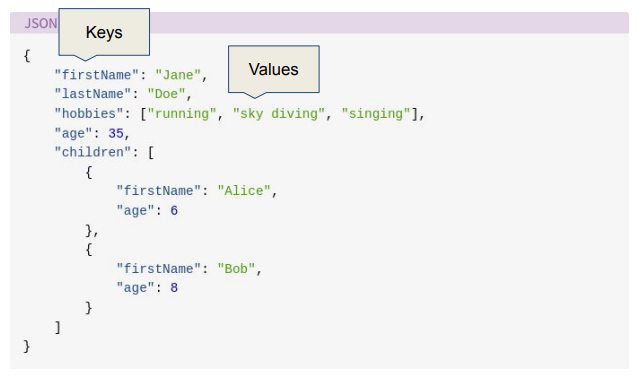
\includegraphics[width = 0.7\textwidth]{figs/json.png}
\caption{Ejemplo de un fichero JSON que describe a una persona. Las llaves representan estructuras y los corchetes listas.}
\label{fig:json}
\end{figure}

Python cuenta con una librería llamada \texttt{json}.
\begin{lstlisting}[language=Python]
import json

json_data =  '{"name":"John", "age":30, "city":"New York"}'

print(json_data)
\end{lstlisting}

%22/10 - Óscar
Para cargar un JSON, se utiliza el método \texttt{json.loads()}. Así, el JSON se guarda en un diccionario que posteriormente se puede guardar serializado en disco. Otra función es \texttt{json.dumps()}, el cual coge un diccionario en una cadena tipo JSON. La función \texttt{json.dump} escribe un objeto JSON en un fichero. 

\begin{table}[htbp]
\centering
\begin{tabular}{l | l}
dict = json.loads(str) & Convierte un string en un diccionario \\
str = json.dumps(dict) & Convierte un diccionario en un string \\
json.dump(dict, file) & Escribe un objeto JSON (dict) en un fichero)
\end{tabular}
\caption{Resumen}
\end{table}

\section{Protocolo HTTP}
Los protocolos de acceso a las bases de datos se han montado sobre el protocolo HTTP. HTTP es un protocolo para obtener recursos en la web, como documentos HTML, imágenes y otros. Es un \textbf{protocolo cliente-servidor}, lo que significa que las peticiones las inicia el destinatario, normalmente el navegador web. 

Una página web es una colección de recursos: imágenes, vídeos, anuncios, etc. Estos elementos pueden estar en sitios distintos, y cuando la página se carga, se embebe en el código y se muestra.
\begin{figure}[htbp]
\centering
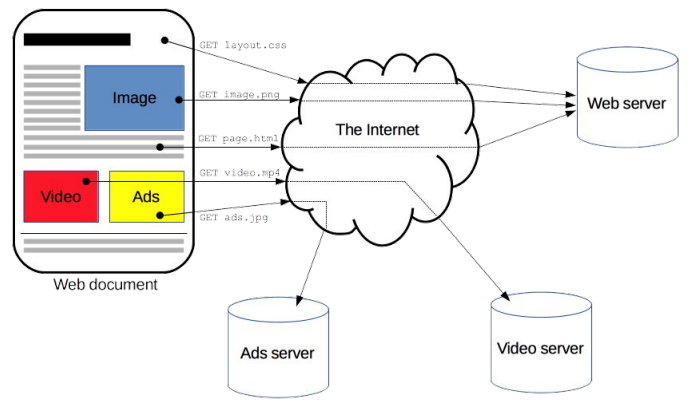
\includegraphics[width = 0.8\textwidth]{figs/web-http.png}
\end{figure}

Los clientes y los servidores se comunican intercambiando mensajes individuales (a diferencia de un flujo de datos). Los mensajes enviados por el cliente, normalmente un navegador web, se denominan \textbf{peticiones (requests)} y los mensajes enviados por el servidor como respuesta se denominan \textbf{respuestas (responses)}.

\subsection{Aspectos básicos de HTTP}
HTTP se diseñó para ser sencillo y legible para los humanos. Los mensajes HTTP pueden ser leídos y comprendidos por humanos, lo que facilita las pruebas a los desarrolladores y reduce la complejidad para los recién llegados. Además, HTTP es extensible: Las cabeceras HTTP hacen que este protocolo sea fácil de ampliar y experimentar. Se pueden introducir nuevas funciones mediante un simple acuerdo entre un cliente y un servidor sobre la semántica de una nueva cabecera.

HTTP no tiene estado, es decir, no existe ningún vínculo entre dos solicitudes que se realizan sucesivamente en la misma conexión. Las cookies HTTP permiten el uso de sesiones con estado (por ejemplo, para utilizar cestas de la compra de comercio electrónico).

\subsection{Flujo HTTP}
Cuando un cliente quiere comunicarse con un servidor realiza los siguientes pasos: 
\begin{enumerate}
\item Abre una conexión TCP: la conexión se utiliza para enviar una petición, o varias, y recibir una respuesta.
\item Envía un mensaje HTTP
\item Espera una respuesta
\end{enumerate}
\begin{figure}[htbp]
\centering
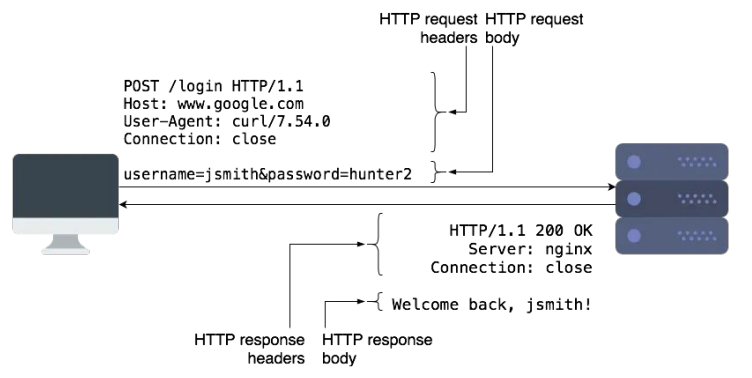
\includegraphics[width = 0.8\textwidth]{figs/http-flow.png}
\end{figure}

Las peticiones son puro texto (no hay datos binarios). La estructura es la siguiente: verbo, url y cabecera para proporcionar información adicional (por ejemplo, el idioma de una página web). La respuesta contiene una línea inicial con el HTTP y un código asociado (200 si todo está bien, 404 si no se ha encontrado, etc), la cabecera y el cuerpo.
\begin{figure}[htbp]
\centering
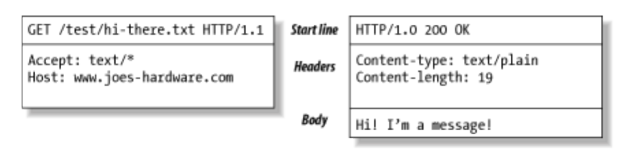
\includegraphics[width = 0.6\textwidth]{figs/request-answer.png}
\end{figure}

Los códigos de retorno son los siguientes:
\begin{table}[htbp]
\centering
\begin{tabular}{c | c | c}
Rango disponible & Rango definido & Categoría \\ \hline
100-199 & 100-101 & Información \\
200-299 & 200-206 & Éxito \\
300-399 & 300-305 & Redirección \\
400-499 & 400-415 & Error del cliente \\
500-599 & 500-505 & Error del servidor 
\end{tabular}
\caption{Códigos de retorno}
\end{table}

Un servidor es un ordenador en un data center. Cada servicio tiene asignado un puerto, ya que en un mismo servidor puede haber varios servicios web. Las direcciones IP (técnicamente IPv4) se dividen en cuatro bloques de tres números que van del 0 al 255 (esto ocupa 8 bites). Así, en el mundo puede haber un máximo de $255^4$ direcciones IP en el mundo. Por ello, a los servicios se les añade después de la dirección IP el puerto. En el caso de la web de la UAM, se trata de 150.244.214.237:80 para HTTP y 150.244.214.237:443 para HTTP. Todos los servicios seguros (HTTPS) se conectan al puerto 443. Una vez conectados al servidor, se puede utilizar el método \texttt{GET} para obtener como respuesta la web que se está pidiendo. Esto se puede realizar en Python con la librería requests y la función get, como se explicó anteriormente. También está el método \texttt{POST} para enviar datos o información a un servidor. Estos datos se incluyen en el cuerpo de la petición, no están visibles en la URL, por lo que se suele utilizar para los login al ser más seguro (usuario y contraseña está oculto a la vista). En resumen: se pide información con GET y se envía información con POST. 

\textbf{Ejemplo: \href{https://rest.ensembl.org/}{https://rest.ensembl.org/}}
Aquí se pueden ver todos los endpoints (las distintas funcionalidades) de la página Ensembl. 
Con \texttt{GET archive/id/:id} se puede acceder a la última versión del identificador que se dé. :id indica la variable que se debería proporcionar, es decir, sustituirlo con el ID. Lo que se devuelve está en formato JSON, pero al leerlo en Python será del tipo string. En este ejemplo, hay un endpoint \texttt{POST archive/id} que lo que hace es devolver la última versión para un conjunto de identificadores. Antes hemos dicho que POST se utiliza para enviar información y GET para obtenerla, pero esta API está mal diseñada y diferencia GET y POST en que el primero es para un solo identificador y el segundo para varios.

En esta página se proponen ejemplos de peticiones. Para GET sería la siguiente:
\begin{lstlisting}[language=Python]
import requests, sys
 
server = "https://rest.ensembl.org"
ext = "/archive/id/ENSG00000157764?"
 
r = requests.get(server+ext, headers={ "Content-Type" : "application/json"})
 
if not r.ok:
  r.raise_for_status()
  sys.exit()
 
decoded = r.json()
print(repr(decoded))
\end{lstlisting}

\subsection{APIs con HTTP}
Los métodos HTTP originales tienen la siguiente semántica:
\begin{itemize}
\item GET: pide obtener una representación del recurso identificado
\item POST: pide añadir información al recurso
\item HEAD: como GET, pero sin recibir el cuerpo, solo la cabecera
\item Otros verbos como DELETE, PUT, CONNECT, TRACE, etc.
\end{itemize}

Para nuestros fines, se utilizará casi siempre GET, pero algunos servidores de datos biomédicos también aceptan POST. Sin embargo, algunos servidores que aceptan POST no lo utilizan para el fin previsto (crear información en el servidor), sino sólo para responder con la representación del recurso (al igual que GET).
URLs como las siguientes utilizan el método GET: \\
\href{https://rest.ensembl.org/sequence/id/ENSG00000157764}{https://rest.ensembl.org/sequence/id/ENSG00000157764} \\
\href{https://www.ebi.ac.uk/Tools/dbfetch/dbfetch?db=uniprot\&id=WAP\_RAT}{https://www.ebi.ac.uk/Tools/dbfetch/dbfetch?db=uniprot\&id=WAP\_RAT}

Un método POST equivalente utiliza una URL sin parámetros (\href{http://rest.ensembl.org/sequence/id/}{http://rest.ensembl.org/sequence/id/}) que se deben enviar junto a los parámetros en el cuerpo de la petición ({"ids":["ENSG00000157764"]}).
\begin{lstlisting}[language=Python]
## GET ##
import requests
gene = "ENSG00000157764"
endpoint = f"http://rest.ensembl.org/sequence/id/{gene}"
r = requests.get(endpoint, headers={ "Content-Type" :"text/plain"})

#Especificando params
gene = "ENSG00000157764"
endpoint = f"http://rest.ensembl.org/sequence/id/{gene}"
parameters = {'species': 'homo_sapiens'}
r = requests.get(endpoint, params = parameters, headers={"Content-Type" : "text/json"})

## POST ##
#Especificando data en lugar de params
response = requests.post(server, data = {'key':'value'})
\end{lstlisting}

\begin{figure}[htbp]
\centering
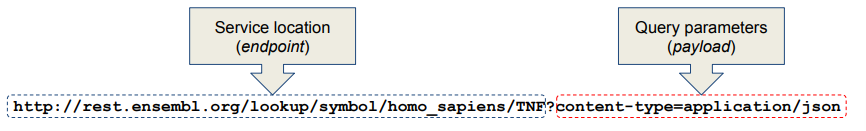
\includegraphics[width = \textwidth]{figs/rest-request.png}
\end{figure}

Aunque las bases de datos sean de acceso público (open access), usualmente piden una API Key, que es un número largo único para cada usuario registrado que se pone en la cabecera. De esa forma, proporcionando el API Key, el servidor sabe qué usuario se está conectando y puede limitar las peticiones de un mismo usuario.

\section{API REST}
REST viene de REpresentational State Transfer. Realmente no es un protocolo, si no un estilo de prestación de servicios web basados en HTTP. 
Los \textbf{servidores} aportan representaciones textuales de recursos (como XML, JSON o HTML), y los \textbf{clientes} piden servicios mediante los métodos HTTP (GET, POST, etc). 
El estado no se guarda en el servidor (cada petición se responde de forma independiente sin memoria de peticiones anteriores).


%29/10 - Gonzalo
\chapter{La línea de comandos de Linux}
\section{Introducción}
\subsection{Test inicial}
La línea de comandos de Linux se puede abrir mediante la combinación de teclas Ctrl + Alt + t. Ejecutamos el siguiente comando: \texttt{wget archive.ics.uci.edu/ml/machine-learning-databases/adult/adult.data}. El comando wget sirve para la descarga no interactiva de ficheros desde la web, soportando los protocolos HTTP, HTTPS y FTP. Con dicho comando, nos decargamos desde la web el fichero adult.data que tiene un tamaño de 3,8 M con permisos de lectura y escritura para el usuario y grupo y solo de lectura para otros. Este fichero contiene datos demográficos de distintas personas, incluyendo la edad, empleo, educación, estado civil, etnia, sexo y país.
\begin{lstlisting}[language=bash]
#Valor del cuarto campo de la tercera fila
cut -d "," -f 4 adult.data | head -n 3 | tail -n 1 #HS-grad

#Cuántas líneas contienen Portugal
grep -c "Portugal" adult.data #37

#Línea en la que aparece Portugal por primera vez
grep -n "Portugal" adult.data | head -n 1 #360

#Valor del primer campo en la fila 1000 empezando por el final
cut -d "," -f 1 adult.data | tail -n 1000 | head -n 1 #40

#Contar el número de filas del fichero
wc -l adult.data #32562

#Crear un fichero con las primeras 1000 filas 
head -n 1000 adult.data > adult-first-1000.data

#Contar bytes del fichero nuevo
wc -c adult-first-1000.data #121895

#Contar las líneas que contienen el string "Married-civ-spouse"
grep -c "Married-civ-spouse" adult.data #14976

#Valor mayor y menor del primer campo
cut -d "," -f 1 adult.data | sort -n | tail -n 1 #90 
cut -d "," -f 1 adult.data | sort -n | head -n 2 #17, hay un blanco
\end{lstlisting}

\subsection{Redirección y tuberías}
Se puede redireccionar la salida a un fichero mediante > y >> para sobreescribirlo o añadirlo respectivamente. 

Con algunas acciones, la línea de comandos se queda bloqueada hasta que termine la tarea (por ejemplo, con gedit). Con Ctrl C se cierra el procedimiento que estaba corriendo y se recupera el control de la consola de comandos, pero los cambios sin guardar se pierden. Por tanto, se puede enviar ese trabajo al background mediante \&. Otra opción es Ctrl Z, que pausa el procedimiento y permite recuperar el control de la consola.

Las tuberías permiten redireccionar la salida de un comando como input de otro sin necesidad de crear ficheros. Estas tuberías pueden ser concatenadas.

\subsection{Filtros}
Un filtro es un programa que lee la entrada estándar, realiza alguna operación sobre ella y saca el resultado por la salida estándar. Normalmente, se combinan con tuberías, y algunos comandos que pueden servir como filtros son \texttt{head, tail, tr, fmt, grep, sort}.

El comando \texttt{tr} \marginpar[\footnotesize tr] \ sirve para traducir o reemplazar. Por ejemplo, \texttt{tr '[0-9]' '*'} reemplaza todos los números por asteriscos. Si se utiliza -d, se borra el parámetro que se le dé en lugar de reemplazarlo. Asimismo, -c sirve para reemplazar todo lo que no entre en el filtro a lo que se le pase como segundo parámetro. Otro argumento opcional es -s, que comprime  una serie de caracteres repetidos.

Los comandos \texttt{head} y \texttt{tail} \marginpar[\footnotesize head \\ tail] \ permiten mostrar las primeras y últimas líneas respectivamente, pero también tienen algunas opciones adicionales. Cuando se utiliza \texttt{-n -100}, se excluyen las últimas 100 líneas, mientras que \texttt{-n +100} hace que empiece en la fila 100. 

El comando \texttt{fmt} \marginpar[\footnotesize fmt] \ permite formatear ficheros para que las líneas sean más pequeñas, recolocar palabras, etc. Por ejemplo, \texttt{fmt -70 -s} hace que cada línea muestre como máximo 70 caracteres, mostrando los caracteres restantes en una nueva línea.

\begin{lstlisting}[language=bash]
#Muestra los 10 procesos más recientes del sistema del usuario actual
ps -ef | tr -s ' ' | grep 'sandra ' | tail -n 10

#Muestra las páginas del manual de grep con 100 caracteres por línea, sustituyendo los dígitos por asteriscos y redireccionando a un fichero
man grep | fmt -100 | tr '[0-9] '*' > file.txt
\end{lstlisting}

El comando \texttt{split} \marginpar[\footnotesize split] \  divide un fichero en distintos bloques de 1000 líneas de forma predeterminada. Ese valor se puede modificar con -l, o se puede definir la cantidad de ficheros de tamaño equitativo sin romper líneas con -n.

El comando \texttt{cut} \marginpar[\footnotesize cut] \ borra secciones de cada línea de un fichero. Con -d se define el delimitador de las distintas columnas, y con -f se selecciona la columna.

El comando \texttt{paste} \marginpar[\footnotesize paste] \ permite combinar varios ficheros que consistan de distintas columnas. Se puede definir el delimitador con -d, que de forma determinada utiliza tabulador. Así, es el comando contrario a cut. 

\begin{lstlisting}[language=bash]
#Extrae las columnas 6 y 4 del fichero adult.data en ese orden.
cat adult.data | cut -d ',' -f 6 > adult-f6.data
cat adult.data | cut -d ',' -f 4 > adult-f4.data
paste -d ',' adult-f6.data adult-f4.data > adult-f6-f4.data
\end{lstlisting}

%31/10 - Gonzalo
Esto puede ser útil para combinar un fichero sin numerar con una columna que contenga la numeración.
\begin{lstlisting}[language=bash]
wc -l adult.data #32562
echo {1..32562} | tr ' ' '\n' > column-numbers.txt
paste -d ',' column-numbers.txt adult.data > adult-numbered.data
\end{lstlisting}

El comando \texttt{shuf} \marginpar[\footnotesize shuf] \  (de shuffle) permite generar permutaciones aleatorias, mezclando o barajando las líneas. Con el parámetro -r, se permiten las repeticiones, y -n permite especificar el número de mezclas.
\begin{lstlisting}[language=bash]
#Mezclar las primeras 10 filas
head adult-numbered.data | shuf
#Mezclar las primeras 5 filas
head adult-numbered.data | shuf -n 5
#Generar 15 filas mezcladas con repetición
head adult-numbered.data | shuf -n 15 -r
#Crear una permutación aleatoria de los números 2 a 9
shuf -i 2-9
\end{lstlisting}
 
 El comando \texttt{sort} \marginpar[\footnotesize sort] \ ordena las filas utilizando ordenación alfabética ASCII (las mayúsculas están por delante de las minúsculas; Z va antes que a). Para ignorar las mayúsculas y minúsculas, se debe poner -f, y para ordenación numérica, -n o -g. 
 
 El comando \texttt{uniq} \marginpar[\footnotesize uniq] \ elimina las filas adyacentes repetidas. Esto se suele utilizar junto a sort para primero ordenar las filas y luego borrar las repetidas. -c indica cuántas filas había de cada tipo. 
\begin{lstlisting}[language=bash]
#Extraer el tipo de región de un fichero GFF y contar cuántas filas hay de cada tipo
cut -f 3 GCF_000002765.3_ASM276v1_genomic.gff | grep -v '#' | sort | uniq -c
#Extraer una lista ordenada de todos los posibles valores del campo 6 de adult.data
cut -f 6 -d , adult.data | sort | uniq -c
\end{lstlisting}

El comando \texttt{join} \marginpar[\footnotesize join] \ une líneas de dos ficheros en base a un campo en común. -1 sirve para especificar el campo del fichero 1, y -2 igual para el segundo fichero. -t permite especificar el delimitador.
\begin{lstlisting}[language=bash]
cut adult-numbered.data -d ',' -f 1,3 | shuf -n 1000 | sort -t ',' -k 1,1 > f13.txt
cut adult-numbered.data -d ',' -f 1,7 | shuf -n 1000 | sort -t ',' -k 1,1 > f17.txt
join -t ',' -1 1 -2 1 f13.txt f17.txt
#Y lo mismo pero manteniendo todas las líneas del primer fichero
join -t ',' -1 1 -2 1 -a 1 f13.txt f17.txt
\end{lstlisting}

El comando \texttt{comm} \marginpar[\footnotesize comm] \ sirve para comparar dos ficheros ordenados de forma alfabética. El resultado son tres columnas. En la primera, se muestran los datos únicos del primer fichero, en la segunda, los datos únicos del segundo, y en la tercera, los datos comunes en ambos ficheros. 

\begin{lstlisting}[language=bash]
#Crea un fichero a.txt con 20 números aleatorios entre 0 y 100 sin repetir; cada número debe estar en una línea distinta
shuf -i 0-100 -n 20 | sort > a.txt
#Crea un segundo fichero b.txt con 20 números aleatorios entre 0 y 100 sin repetir; cada número debe estar en una línea distinta
shuf -i 0-100 -n 20 | sort > b.txt
#Muestra los números que aparezcan en ambos ficheros
join -t ',' -1 1 -2 2 a.txt b.txt
comm -12 a.txt b.txt
\end{lstlisting}

\subsection{Scripts de shell}
Todos los comandos vistos anteriormente se pueden utilizar en scripts de bash. Los script deben empezar con el intérprete.
\begin{lstlisting}[language=bash]
#!/bin/bash
#Hello world script

echo "Hello World!"
\end{lstlisting}

Para ejecutar un script, primero se le debe dar permisos de ejecución mediante \texttt{chmod +x hello-world.sh}. Dentro de un fichero se pueden crear variables asignando el valor con el igual sin dejar espacios. Para luego poder llamar a la variable, se debe llamar con un \$ delante del nombre.

\begin{lstlisting}[language=bash]
#!/bin/bash
#Variables:
input_file='adult.data'
output_file='adult5-7.data'
fields='5-7'

#Remove spaces and get selected fields:
cat $input_file | tr -d ' ' | cut -d ',' -f $fields > tmp.txt

#Sort and get unique lines:
sort tmp.txt | uniq > $output_file

#Remove temporary file:
rm tmp.txt
\end{lstlisting}

También es posible introducir argumentos a un script, los cuales se llaman con \$1-9. \$0 representa el nombre del fichero.
\begin{lstlisting}[language=bash]
#!/bin/bash
#Remove spaces and get selected fields:
cat $1 | tr -d ' ' | cut -d ',' -f $3 > tmp.txt

#Sort and get unique lines:
sort tmp.txt | uniq > $2

#Remove temporary file:
rm tmp.txt

#Show head of new file:
head -n 20 $2
\end{lstlisting}

Ejercicio: escribir un script que acepte tres argumentos: f, a, b. El argumento f es el nombre de un fichero csv, y los argumentos a y b son números integer. El script debe mostrar la lista de valores coincidentes en las columnas a y b del fichero f.
\begin{lstlisting}[language=bash]
#!/bin/bash
file=$1
column1=$2
column2=$3

cut -d ',' -f $column1 $file > tmp1.txt
cut -d ',' -f $column2 $file > tmp2.txt
join -t ',' -1 1 -2 1 tmp1.txt tmp2.txt

rm tmp1.txt tmp2.txt
\end{lstlisting}

\subsection{Editores de texto}
\texttt{vi} es un editor de texto que viene en todas las distribuciones de Linux. La ventaja es que no abre ventanas externas (como gedit). Tiene dos modos: modo de inserción y modo de comando. En modo comando, los caracteres que se pulsan se interpretan como comandos, y se puede navegar mediante hjkl. Pulsando i, se cambia al modo de inserción, pudiendo añadir texto al editor. Para salir sin guardar, se debe poner \texttt{:q!}, y para salir guardando, \texttt{:x}. Para volver al modo de comando desde el modo inserción, basta con pulsar Esc. 

\section{Expresiones regulares y grep}
El comando \texttt{grep} permite buscar texto, pero también patrones. Los patrones emplean distintos símbolos:
\begin{itemize}
\item $\wedge$ : inicio (por ejemplo, "$\wedge$Hola")
\item \$: final (por ejemplo, "Pepito\$")
\item .: comodín, cualquier carácter (por ejemplo, "Pepit." encuentra tanto Pepito como Pepita).
\item \lbrack \rbrack: indican un conjunto de caracteres válidos ("Pepit[ao]" encuentra Pepito y Pepita, pero no Pepite).
\item \lbrack  $\wedge$ \rbrack : en la posición de los corchetes, vale cualquier carácter menos los que se especifiquen dentro ("Pepit[$\wedge$o]" solo encuentra Pepita).
\item *: indica un número indeterminado de repeticiones del carácter anterior, siendo 0 una posibilidad. Por ejemplo, con la expresión "[1-9][0-9]*th", se encontrarían 01th, 15th, 2th y 2333th. De 01th, solo se encontraría 1th con el patrón, ya que el 0 no está incluido en el primer conjunto. Así, tanto 01th como 2th tienen el dígito en el primer corchete, el segundo corchete se repite 0 veces y finaliza en th. En el caso de 2333th, el 2 se encontraría en el primer corchete, y los 3 en el segundo corchete, repitiéndose las veces necesarias. 
\end{itemize} 

Una expresión regular que extraiga las líneas que contengan solo números sería la siguiente:
\begin{lstlisting}[language=bash]
#! /bin/bash
grep "^[0-9]*[0-9 ,]*$" $1
\end{lstlisting}

\end{document}
